% !TEX options=--shell-escape
\documentclass[usenames,dvipsnames,9pt]{beamer}

\makeatletter
\def\input@path{{support/beamer-template/}}
\makeatother

\usepackage{support/beamer-template/beamerthememetropolis}

\usepackage[utf8]{inputenc}
\usepackage[czech]{babel}
\selectlanguage{czech}

\usepackage{hyperref}
\usepackage{fontawesome}
\usepackage{minted}
\usepackage{mathtools}
\usepackage{tabularx}
\usepackage{smartdiagram}
\usepackage{amssymb}
\usepackage{qrcode}

% Commands shared between most of the tutorial slides

% Homework deadlines
\newcommand{\hwVIIdeadline}{10. 5. 2020}



% Download icon and text with link relative to the root of the courseware site
\newcommand{\download}[1]{\hfill\faDownload\hspace{5pt}\href{https://cw.fel.cvut.cz/wiki/_media/courses/be4m36mas/#1}{\tt #1}\\[1.3em]}

% Draw eye icon
\newcommand{\see}[1]{\faEye\hspace{5pt}#1}

\newcommand{\sep}{\hspace{10pt}/\hspace{10pt}}

\def\Ipe#1{\def\IPEfile{#1}\input{#1}}

% Draw pacman icon
\newcommand{\pacman}[1]{\tikz[baseline=.1em,scale=.6]{
    \useasboundingbox (.02,0) rectangle (.6,.6);
  \draw [fill=#1] (.3,.3) -- ++(25:.3) arc (+25:+335:.3) -- cycle;

}}

% Draw ghost icon
\newcommand{\ghost}[1]{\tikz[baseline=.1em,scale=.5]{
  \draw [fill=#1] (0,0) -- (0,.5) arc (+180:0:.3) -- (.6,0) --
  (.5,.15) -- (.4,0) -- (.3,.15) -- (.2,0) -- (.1,.15) -- cycle;
    \coordinate (eye) at (360*rand:.03);
    \foreach \x in {.17,.43}{
      \fill[white] (\x,.5) circle[radius=.1];
      \fill[black] (\x,.5) ++(eye) circle[radius=.05];
    }
}}

\newcommand{\desc}[2]{
  #1

  \vspace{-0.6em}
  \hfill\begin{minipage}{0.9\linewidth}
    #2
  \end{minipage}

  \vspace{0.2em}
}

\newcommand{\redc}{\tikz\draw[red,fill=red] (0,0) circle (.5ex);}

\newcommand{\greenc}{\tikz\draw[green,fill=green] (0,0) circle (.5ex);}


% Default url for generating QR code with feedback form.
\newcommand{\defaultfeedbackurl}{https://forms.gle/vwbWazEu14w1Kf487}

% Generate frame with QR code to a feedback form.
\newcommand{\framefeedback}[1][\defaultfeedbackurl]{
  \begin{frame}[standout]
    \begin{minipage}{0.4\linewidth}
      \begin{center}
        \textbf{\LARGE Díky za pozornost!}
      \end{center}

      \vspace{3em}

      \raggedleft\small Budeme rádi za Vaši\\zpětnou vazbu! $\rightarrow$
    \end{minipage}
    \hfill
    \begin{minipage}{0.5\linewidth}
      \vspace{4em}
      \centering\qrcode[height=\linewidth]{#1}\\
      \vspace{0.8em}
      \url{#1}
    \end{minipage}
  \end{frame}
}

\title{Dekompoziční techniky}
\date{}
\institute{B4B36PDV -- Paralelní a distribuované výpočty}

\metroset{block=fill}

\begin{document}
\maketitle


%\begin{frame}[t]
%  Minulé cvičení:
%  \begin{center}
%    \Large\emph{``Konkurentní datové struktury...''}
%  \end{center}
%  
% % \pause
%
%\begin{figure}
%  \only<2>{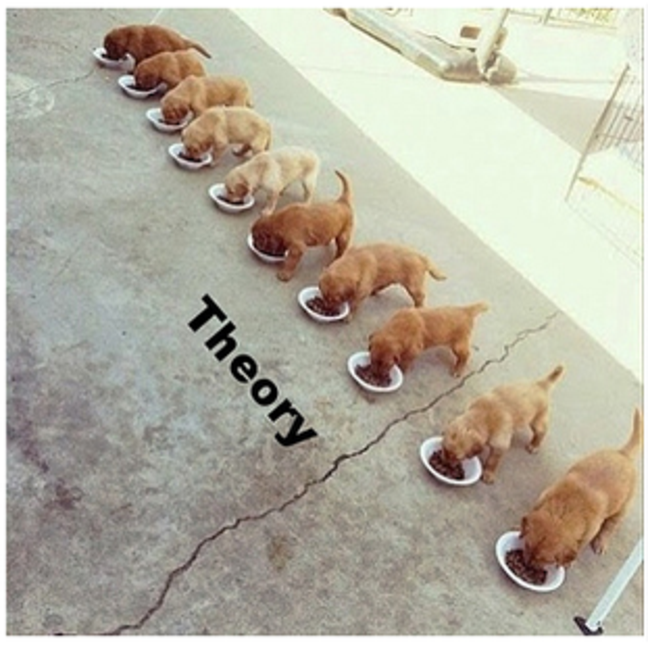
\includegraphics[scale=0.4]{05/figs/theory.pdf}}%
%  \only<3->{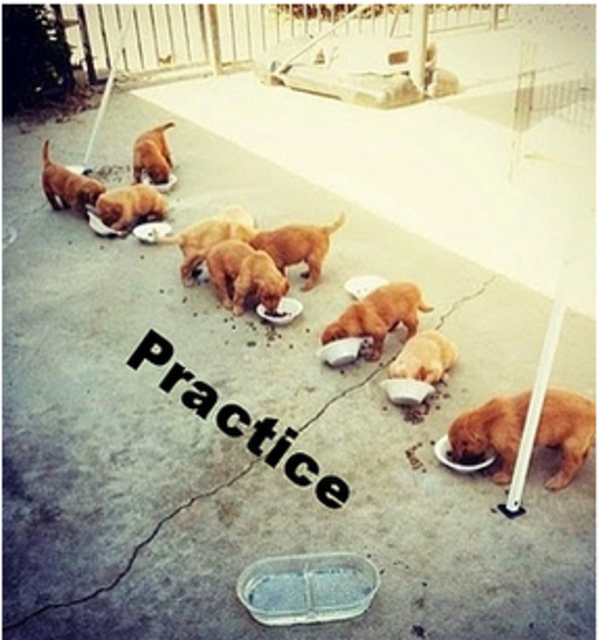
\includegraphics[scale=.4]{05/figs/practice.pdf}}%
%\end{figure}
%
%\pause
%
%  \only<4>{Dnešní menu: \hspace{10pt} \huge Dekompoziční techniky}
%\end{frame}

\begin{frame}
  \frametitle{Osnova}
  \begin{itemize}
    \item Opakování z minulého cvičení
    \item Datová dekompozice se zařezáváním
    \item Explorativní dekompozice
    \item Rekurzivní dekompozice\\[1.5em]
    \item Zadání čtvrté domácí úlohy
  \end{itemize}
\end{frame}

\section{Opakování z minulého cvičení}
\begin{frame}[standout]
  \Huge
  \url{http://goo.gl/a6BEMb}
\end{frame}

\begin{frame}[fragile]

\frametitle{Jakým způsobem bude následující kód proveden?}

	\begin{minted}{c}
	int a = getCurrentValue();
	int b = compute(); // casove narocna funkce
	int c = getCurrentValue();
	if (a < b){
		a.compare_exchange_strong(c, b);
	}
	\end{minted}
	
	\vspace{2em}
	\begin{itemize}
	\item Kód nelze zkompilovat
	\item Do A se vždy uloží B
	\item Do A se uloží C, pokud B není rovno C
	\item Do C se uloží A, pokud A není rovno B
	\item Do A se uloží B, pokud A není rovno C
	\item Kód vrací chybu, pokud A není rovno C
	\end{itemize}

\end{frame}

\begin{frame}[fragile]

\frametitle{V čem může být rozdíl po ukončení výpočtu následujících dvou funkcí?}

	\begin{minted}{c}
void compute_1(){
	node * null_ptr = nullptr;
	node * a = getMainNode();
	if(a == null_ptr){
		if(getMainNode().compare_exchange_strong
			(null_ptr, getNewNode())){ 
				return;
		}}
	std::cout << a->value << std::endl;}
	
void compute_2(){
	node * null_ptr = nullptr;
	node * a = getMainNode();
	if(a == null_ptr){
		if(getMainNode().compare_exchange_strong
			(a, getNewNode())){ 
				return;
		}}
	std::cout << a->value << std::endl;}
	\end{minted}

\end{frame}

\section{Cvičení: Problém $3n+1$}

\begin{frame}
	\frametitle{Problém $3n+1$ (Collatzův problém)}
	Collatzova posloupnost je definovaná následovně (pro $n \in \mathbb{N}$):
	\[
		f(n) = \begin{cases}
			n/2  & \text{pro $n$ sudé} \\
			3n+1 & \text{pro $n$ liché}
		\end{cases}
	\]
	Příklad pro počáteční $n=5$:
	\begin{center}
		\LARGE 5\ \ \  16\ \ \  8\ \ \  4\ \ \  2\ \ \  1\ \ \  4\ \ \  2\ \ \  1\ \ \  4\ \ \  2\ \ \  1 ...
	\end{center}

	\pause

	\vspace{1em}\hrule\vspace{1em}

	Má se za to, že tato sekvence vždy dosáhne \textbf{1} (\emph{Collatz conjecture}).\\
	Po kolika krocích se tak ale stane?

	{
		\hfill
		\Large Collatzova funkce $C(n)$
	}

	{
		\hfill
		např. $C(5)=5$, $C(16)=4$
	}

\end{frame}

{\setbeamertemplate{frame footer}{\see{{\tt decompose.cpp}, {\tt main.cpp}}}
\begin{frame}[fragile]
	\frametitle{Problém $3n+1$ (Collatzův problém)}
	Úkol 1: Máme zadanou konečnou podmnožinu přirozených čísel $X \subset \mathbb{N}$. Jaké je minimum funkce $C(n)$ na množině $X$?
	\[ \min_{n \in X} C(n) \]
	\pause
  \begin{center}
    \Large Jak výpočet optima paralelizovat?
  \end{center}
  \pause
  \begin{center}
    {\Large Jak paralelní výpočet zrychlit?}
    Musíme vždy generovat celé sekvence?
  \end{center}

  \pause
  \begin{block}{Doimplementujte metodu \texttt{findmin\_parallel}}
    Doimplementujte tělo metody \texttt{findmin\_parallel} v souboru \texttt{decompose.cpp} pro paralelní nalezení optima $C(n)$ na množině $X$ (reprezentované vektorem \texttt{data}).
    Udržujte si dosud nalezené optimum pro zařezávání nepotřebných výpočtů $C(n)$ (tj., ve chvíli, kdy daný výpočet prokazatelně vede k suboptimálnímu řešení).
  \end{block}
\end{frame}

\begin{frame}[fragile]
	Úkol 2: Nalezněte číslo $n \in \mathbb{N}$ takové, že $C(n) \geq k$.

	\pause
	\vspace{1em}\hrule\vspace{1em}
	Sekvenčně je to jednoduché:
	\begin{minted}{c}
		unsigned long i = 1;
		while(collatz(i) >= k) i++;
	\end{minted}
	\begin{center}
		\Large Jak tento výpočet zparalelizujeme?
	\end{center}

	\pause
	\begin{block}{Doimplementujte metodu \texttt{findn\_parallel}}
		Doimplementujte tělo metody \texttt{findn\_parallel} pro paralelní nalezení čísla $n$, pro které platí $C(n) \geq k$.
	\end{block}
\end{frame}
}

\begin{frame}
	\frametitle{Explorativní dekompozice}
	\faWarning \hspace{3pt}
	Pokud \emph{explorujeme} prostor možných řešení a testujeme, zda existuje prvek, který splňuje nějakou podmínku, chceme výpočet ukončit okamžitě po nalezení prvního vhodného prvku.

	\pause
	\vspace{0.5em}
	\hfill V případě paralelizace výpočtu chceme ukončit \underline{všechna} vlákna!
\end{frame}

% {\setbeamertemplate{frame footer}{\see{{\tt decompose.cpp}, {\tt main.cpp} \sep {\tt make main}}}
% \begin{frame}[fragile]
% \frametitle{Collatzův problém}
% Collatzova funkce je definována následovně:

% \vspace{1em}

% \begin{math}
% C(n) = 
% \begin{cases}
%       1 & \text{pokud}\ n = 1 \\
%       1 + C(n/2), & \text{pokud}\ n \equiv 0~(mod~2) \\
%       1 + C(3n+1), & \text{pokud}\ n \equiv 1~(mod~2)
%     \end{cases}
% \end{math}

% \vspace{2em}

% Domněnka je taková, že pro každé $n$ výpočet konverguje v konečném čase.

% Výpočet navíc konverguje monotónně, tedy v každém kroku výpočtu známe $k \leq C(n)$.

% \vspace{1em}

% Př. $C(3) = 1 + C(10) = 2 + C(5) = 3 + C(16) = 4 + C(8) = 5 + C(4) = 6 + C(2) = 7 + C(1) = 8$

% \vspace{1em}

% Hledáme \textbf{minimum} této funkce na dané podmnožině přirozených čísel.
% \end{frame}
% }

% \begin{frame}[fragile]
%   \begin{center}
%     \Large Jak výpočet optima paralelizovat?
%   \end{center}
%   \pause
%     \begin{center}
%     \Large Jak paralelní výpočet zrychlit?
%   \end{center}
  
%     \pause\vspace{2em}
    
%   \begin{center}
%     Využijeme monotonicity $\rightarrow$ sdílení mezivýsledků!
%   \end{center}

% \end{frame}

% \section{Datová dekompozice se zařezáváním}

% {\setbeamertemplate{frame footer}{\see{{\tt decompose.cpp}, {\tt main.cpp} \sep {\tt make main}}}
% \begin{frame}[fragile]


% Se statickou a dynamickou dekompozicí jste se již setkali.

%   \begin{minted}{c}
%  #pragma omp parallel for schedule(static) // schedule(dynamic)
%  for(int i = 0; i < data.size(); i++){
%  	value = collatz(i);
%  	if ( value < min) value = min;
%  }
%   \end{minted}
  
%   \pause\vspace{1em}\hrule\vspace{1em}
  
%   Jak použít mezivýsledky pro rychlejší počítání Collatzovy funkce?
%   \begin{itemize}
%       \item \textbf{Algoritmus si pamatuje aktuální optimum:}\\
%           Update lze provádět pomocí ``porovnej a prohoď''
%     \item \textbf{Ukončení když počet kroků je větší než aktuální optimum:}\\
%           Díky monotonicitě už jsme si jistí, že aktuální hodnota není optimem.
%   \end{itemize}
  


%   \pause\vspace{1em}
  
%   \begin{block}{Doimplementujte metodu \texttt{findmin\_parallel}}
%     Doimplementujte tělo metody \texttt{findmin\_parallel} v souboru \texttt{decompose.cpp}.
%     Pro synchronizaci vláken použijte \texttt{X.compare\_exchange\_strong( T\& expected, T desired)} metodu.
%   \end{block}
% \end{frame}
% }

% \begin{frame}[fragile]
%   \begin{center}
%     \Large Co když nechceme přesné optimum, ale jen $n : C(n)\geq k$?
%   \end{center}
  
%     \pause\vspace{2em}
    
%   \begin{center}
%     Po nalezení můžeme všechny ostatní běžící procesy ukončovat.
%   \end{center}

% \end{frame}

% \section{Explorativní dekompozice}

% \begin{frame}[fragile]

% Vhodná při prohledávání, kdy se jen snažíme splnit lokální podmínku

% Např. existence určitého prvku, daný prvek je dělitelný, našli jsme řešení,...

% \vspace{2em}

% [OBRAZEK]

% [\url{http://parallelcomp.uw.hu/files/03fig07.jpg}]

  
  
% \end{frame}

\begin{frame}[t]
	\frametitle{Explorativní dekompozice: Řešení problému SAT}

	Chceme splnit booleovskou funkci $\phi$ nad booleovskými proměnnými $x$, $y$, $z$, ...
	\begin{figure}
		\centering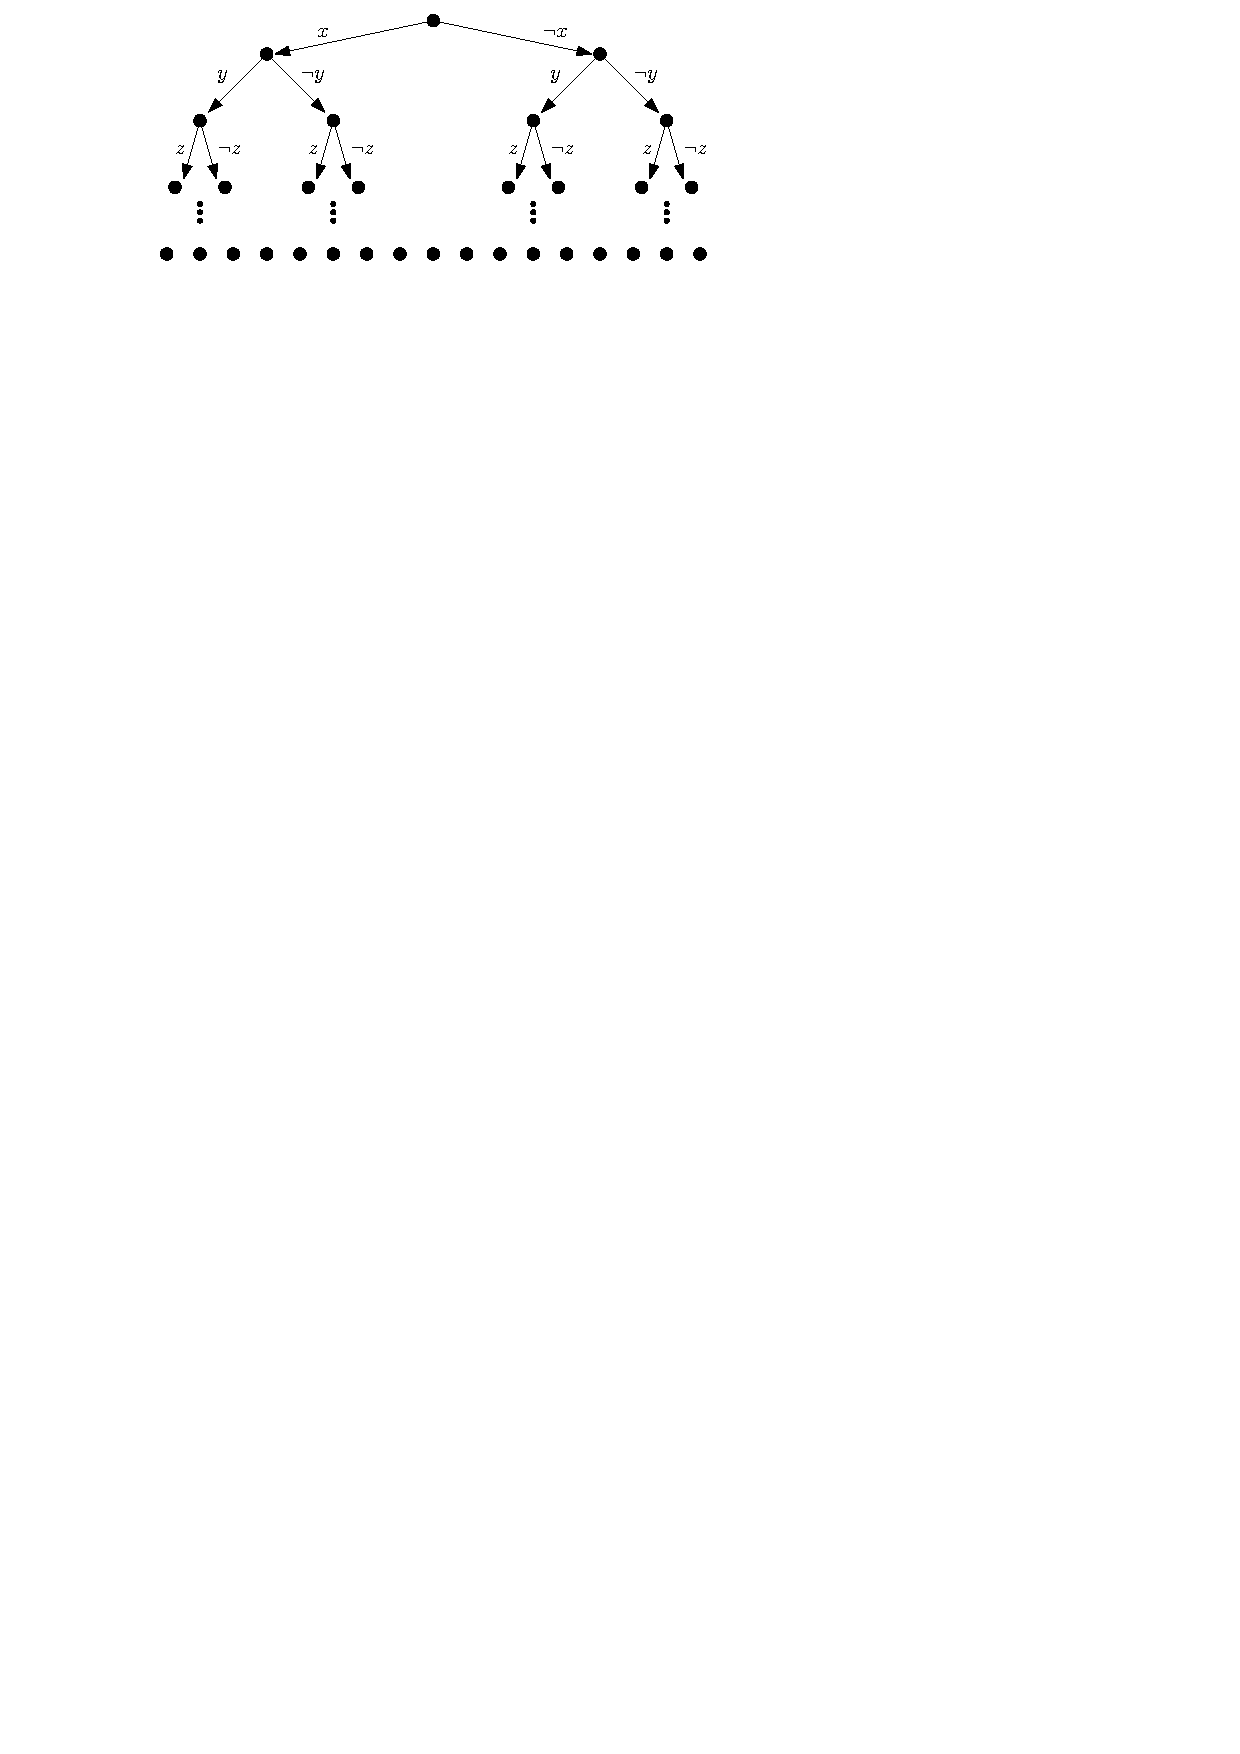
\includegraphics[width=0.8\linewidth]{05/figs/sat1.pdf}
	\end{figure}

	\vspace{1em}
	\begin{center}
		\Large Máme 4 vlákna -- jak byste úlohu paralelizovali?
	\end{center}
\end{frame}

\begin{frame}[t]
	\frametitle{Explorativní dekompozice: Řešení problému SAT}

	Chceme splnit booleovskou funkci $\phi$ nad booleovskými proměnnými $x$, $y$, $z$, ...
	\begin{figure}
		\centering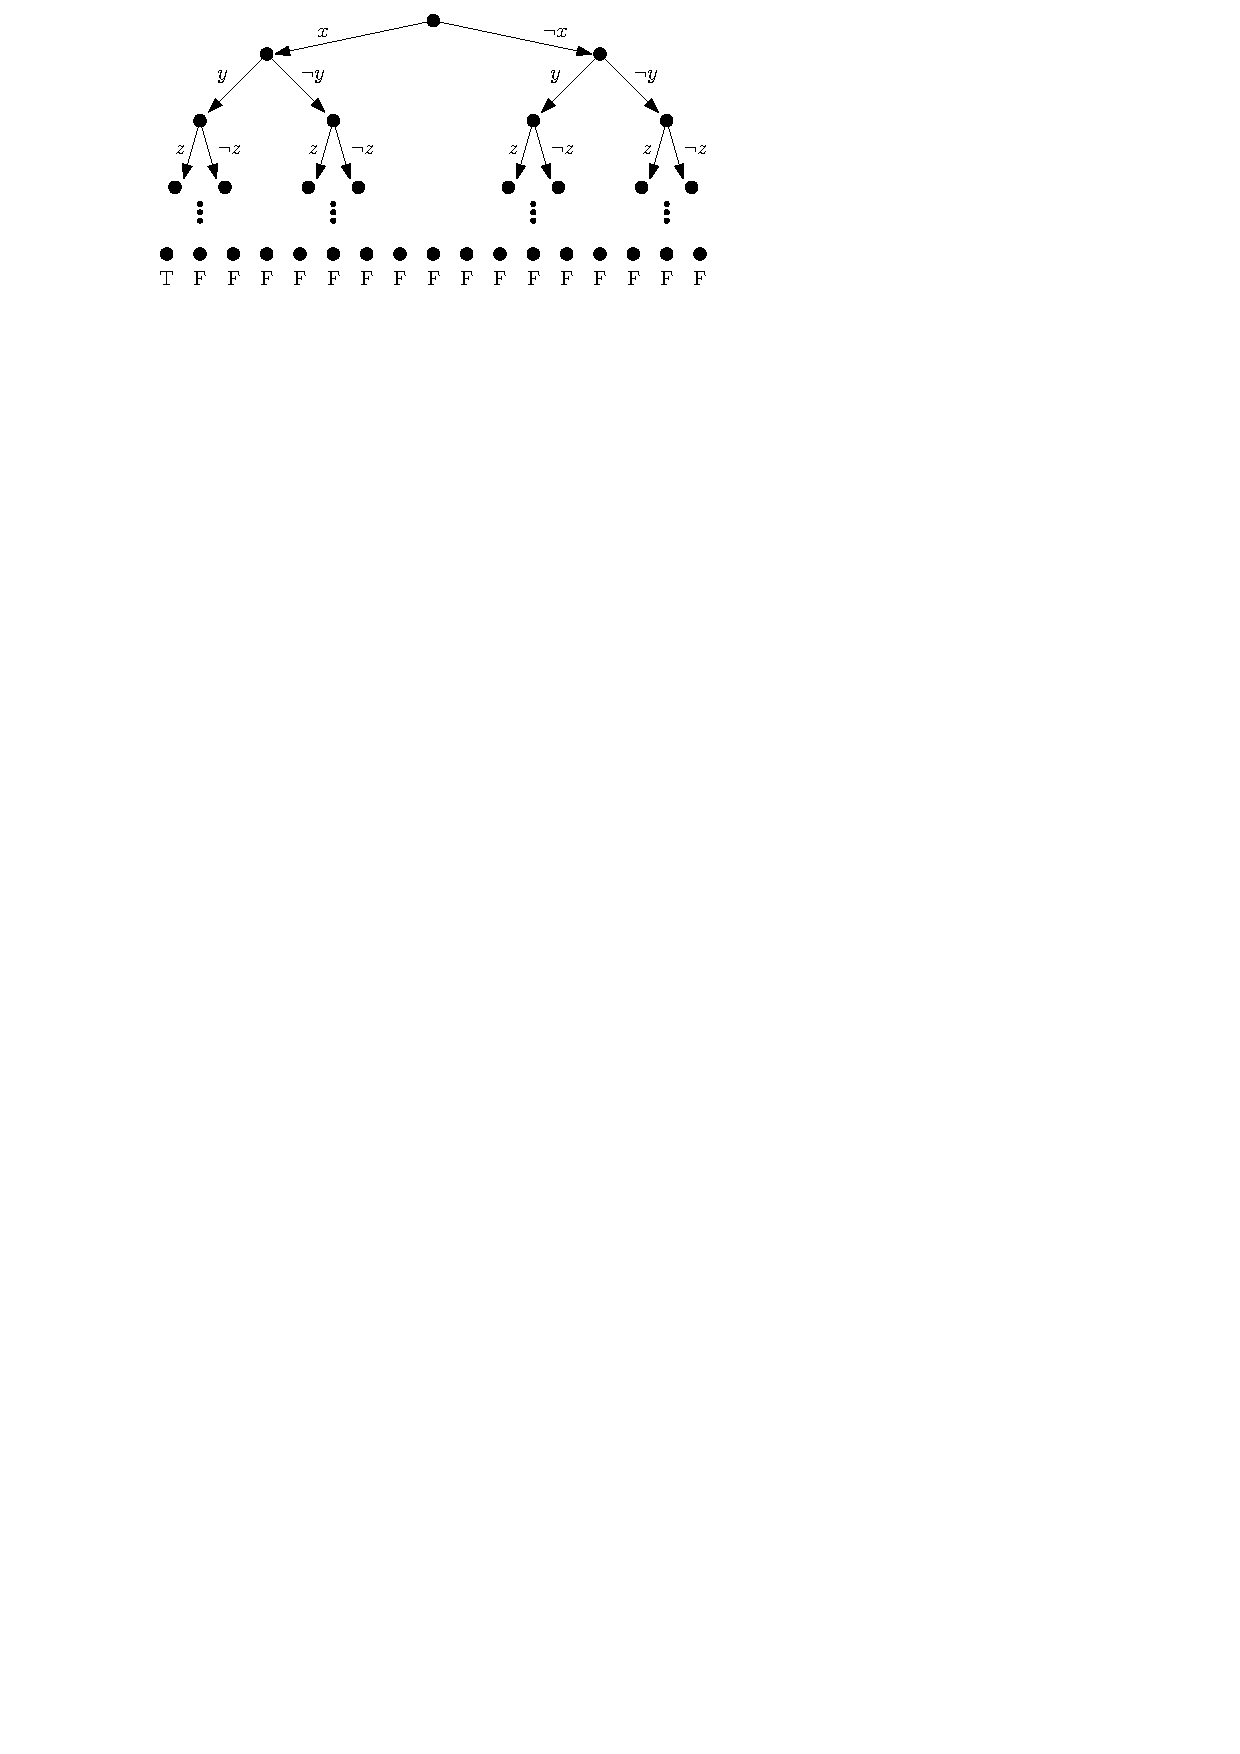
\includegraphics[width=0.8\linewidth]{05/figs/sat2.pdf}
	\end{figure}
\end{frame}

{\setbeamertemplate{frame footer}{\see{{\tt decompose.cpp}, {\tt main.cpp}}}
\begin{frame}[fragile]
	\frametitle{Jak na to?}

  \begin{minted}{c}
#pragma omp parallel
#pragma omp for
for (...){
    if (condition){
    	#pragma omp cancel for 
    }
}
  \end{minted}
\end{frame}

\begin{frame}[fragile]
	\frametitle{Jak na to?}
  \begin{minted}{c}
#pragma omp parallel
{
  while(true){
   #pragma omp cancellation point parallel
    if (condition){
    #pragma omp cancel parallel
    }
  }
}
  \end{minted}
  
  \vspace{1em}
  {\Large \faWarning \hspace{3pt} Nutné nastavit v prostředí \texttt{\textbf{OMP\_CANCELLATION = true}} !}

  
  
\end{frame}
}

\begin{frame}[fragile]
	\frametitle{Rekurzivní dekompozice}

	\text{\Large Z algoritmizace víte, že pro některé úlohy je vhodná rekurze.}

	\hfill Vzpomeňte si na řazení! (např. quick-sort z přednášky)

	\begin{figure}
		\centering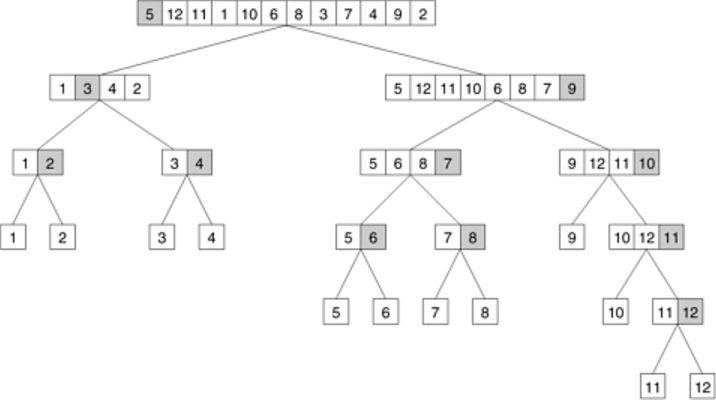
\includegraphics[width=0.7\linewidth]{05/figs/quicksort.png}
	\end{figure}

	\pause\vspace{2em}

	\begin{center}
		{\Large Jak takovýto rekurzivní výpočet zparalelizovat?}\\
		U rekurzivních úloh často ani nevíme, jaké podúkoly budeme muset řešit...
	\end{center}
\end{frame}

\begin{frame}
	\frametitle{Rekurzivní dekompozice}

	{\Large Řešení: Budeme paralelní úlohy spouštět dynamicky!}

	\hfill\begin{minipage}{0.8\linewidth}
	  Ve chvíli, kdy potřebujeme zavolat jinou rekurzivní metodu spustíme nový \texttt{\#pragma omp task}.
	  Ten se zpracuje ve chvíli, kdy nějaké vlákno nemá, co dělat.
	  Vzpomeňte si na thread-pool!
  \end{minipage}

  \pause
  \vspace{2em}\hrule\vspace{2em}

  Otázka: Jak se tento přístup liší od \texttt{\#pragma omp parallel for schedule(dynamic)}?
\end{frame}

\begin{frame}[fragile]
\frametitle{Příklad \texttt{\#pragma omp task}: Paralelní suma}

\begin{minted}{c}
float sum(const float *a, size_t n){
    float r;
    #pragma omp parallel
    #pragma omp single
    r = parallel_sum(a, n);
    return r;
}

static float parallel_sum(const float *a, size_t n){
    if (n <= CUTOFF) { return serial_sum(a, n);}
    float x, y;	size_t half = n / 2;
    #pragma omp task shared(x)
    x = parallel_sum(a, half);
    #pragma omp task shared(y)
    y = parallel_sum(a + half, n - half);
    #pragma omp taskwait
    x += y;
    return x;
}
  \end{minted}
  
\end{frame}


{\setbeamertemplate{frame footer}{\see{{\tt decompose.cpp}, {\tt main.cpp}}}
\begin{frame}[fragile]
\frametitle{Fibonacciho posloupnost}

\[
1,\ \  1,\ \  2,\ \  3,\ \  5,\ \  8,\ \  13,\ \  21,\ \  34,\ \  55,\ \  89,\ \  144,\ \  233,\ \  377,\ \  610, ...
\]

Fibonacciho posloupnost (pro $n \in \mathbb{N}$) je definovaná:

\[
F(n) = 
\begin{cases}
      1 & \text{pokud $n = 1$ nebo $n=2$} \\
      F(n-1) + F(n-2), & \text{jinak}
    \end{cases}
\]

\vspace{2em}

	\pause

  \begin{block}{Doimplementujte metodu \texttt{fibonacci\_parallel\_worker}}
    Doimplementujte tělo metody \texttt{fibonacci\_parallel\_worker} v souboru \texttt{decompose.cpp}.
    Rekurzivní volání spouštějte pomocí direktivy \texttt{\#pragma omp task}.
  \end{block}

  \begin{center}
  	\large \faWarning \hspace{3pt} Proměnné v \texttt{task} jsou privátní (\texttt{lastprivate}) pro daný task, pokud neřeknete jinak (pomocí parametru OpenMP \texttt{shared(x)}).
  \end{center}
\end{frame}
}


% \section{Zadání čtvrté domácí úlohy}

% \begin{frame}[fragile]
%   \frametitle{Paralelní dotazy do databáze}
  

% \end{frame}

% \begin{frame}
%   \frametitle{Paralelní dotazy do databáze}
%   Naimplementujte metody v \texttt{-.cpp} a zajistěte, že
% %  \begin{enumerate}
% %    \item každý prvek je vložet právě jednou; a
% %    \item žádný vložený prvek se neztratí.
% %  \end{enumerate}
  
  
%   \vspace{1.5em}
  
%   Za správné výsledky a rychlé zpracování dostanete až {\bf 2b}.
  
%    \vspace{1.5em}
    
%   \begin{tabbing}
%   Termín odevzdání je \={\bf 29.3. 23:59 CET} pro středeční cvičení a\\
%   \>{\bf 30.3. 23:59 CET} pro čtvrteční cvičení.
% \end{tabbing}

% Soubor \texttt{-.cpp}  nahrajte do systému BRUTE.
  

% \end{frame}


% Frame with the feedback QR code 
\framefeedback{}



\end{document}
